% !TeX program = XeLaTeX
\documentclass[a4paper,11pt]{article}

% Essential packages
\usepackage[top=25mm, bottom=25mm, left=20mm, right=20mm, columnsep=8mm]{geometry}
\usepackage{amsmath,amsthm,amssymb,mathtools}
\usepackage{graphicx}
\usepackage{booktabs}
\usepackage{longtable}
\usepackage{setspace}
\usepackage{algorithm}
\usepackage{algorithmic}
\usepackage{listings}
\usepackage[table]{xcolor}
\usepackage{subcaption}
\usepackage{float}
\usepackage{multirow}
\usepackage{array}
\usepackage{threeparttable}
\usepackage{url}

% Bibliography with biber
\usepackage[backend=biber,style=numeric,sorting=none]{biblatex}
\addbibresource{SBUKThesis-bibliography.bib}

% Color definitions
\definecolor{Blue}{rgb}{0,0,0.55}
\definecolor{mybluecolor}{HTML}{80C4E9}

% Hyperref package
\usepackage[colorlinks=true,
            linkcolor=black,
            citecolor=black,
            urlcolor=black,
            filecolor=black,
            menucolor=black,
            runcolor=black,
            linktoc=all,
            pdfstartview=FitH,
            breaklinks=true]{hyperref}

% Font settings
\usepackage{fontspec}
\setmainfont{Times New Roman}

% Line spacing
\linespread{1.5}

\begin{document}

% Title and authors
\title{\Large\textbf{MAGNET: A Multi-modal Deep Learning Framework for Android Malware Detection Using Transformers and Graph Neural Networks}}
\author{
  \textbf{Alireza Iranmanesh}\thanks{Shahid Bahonar University, Master's student in Artificial Intelligence, Kerman, Iran. Email: alirezairanmanesh78@gmail.com} \and
  \textbf{Dr. Hamid Mirvaziri}\thanks{Shahid Bahonar University, Computer Engineering Department, Kerman, Iran. Email: h.mirvaziri@gmail.com}
}
\maketitle
\vspace{-1em}

% Abstract
\begin{abstract}

\textbf{Background and Motivation:} Android malware detection is becoming a major challenge in information security due to the increasing cyber threats. Traditional methods, especially those relying solely on single-modal feature analysis, often face limitations such as the inability to process complex multi-modal data and poor generalization to new threats. These shortcomings highlight the need for developing novel and efficient approaches.

\textbf{Method and Approach:} We propose MAGNET (Multi-modal Analysis for Graph-based NEtwork Threats), a multi-modal deep learning framework that leverages a combination of tabular, graph, and sequential data—such as API call sequences—for Android malware detection. The architecture comprises three specialized components: (1) \textit{EnhancedTabTransformer} for static feature analysis; (2) \textit{GraphTransformer} for function call relationship modeling using graph neural networks; and (3) \textit{SequenceTransformer} for temporal API invocation pattern recognition. A dynamic attention mechanism with learnable fusion weights optimally combines multi-modal representations for final classification.

\textbf{Experimental Design:} The model was trained on the DREBIN dataset consisting of 4,641 training samples and 1,451 test samples, with 5-fold cross-validation. Hyperparameter optimization was performed using advanced algorithms including PIRATES (476 trials) and Optuna (13 trials). The final model used single-layer transformers with embedding dimensions of 32-64, 4 attention heads, and dynamic fusion mechanisms.

\textbf{Results and Performance:} MAGNET achieves exceptional performance with 97.24\% accuracy, F1-score of 0.9823, precision of 0.9796, recall of 0.9849, and AUC of 0.9932. In 5-fold cross-validation, the model demonstrates consistent performance with accuracy 97.22±0.65\%, F1-score 98.18±0.42\%, and AUC 99.32±0.35\%. Component analysis shows individual contributions: EnhancedTabTransformer (F1: 0.945), GraphTransformer (F1: 0.894), and SequenceTransformer (F1: 0.907). The model significantly outperforms baseline methods including SVM (90.6\%), Random Forest (93.5\%), XGBoost (94.8\%), and ANN (96.2\%).

\textbf{Significance and Impact:} This work establishes a comprehensive evaluation of transformer-based multi-modal architectures for Android malware detection, demonstrating that synergistic integration of heterogeneous data modalities substantially enhances detection capabilities. The framework's superior performance and interpretability make it suitable for deployment in production security systems.

\textbf{Keywords:} Android malware detection, Multi-modal deep learning, Graph neural networks, Transformer architecture, Attention mechanisms, Cybersecurity, DREBIN dataset

\end{abstract}

\newpage
\twocolumn

\section{Introduction}
Android's dominance in the mobile ecosystem is undeniable, commanding over 70\% of the global smartphone market and establishing itself as the world's most prevalent mobile platform~\cite{AndroidSecurity}. However, this remarkable success has an unfortunate counterpart: Android's open architecture and widespread deployment have inevitably attracted malicious actors. The Android malware landscape has witnessed exponential growth, with sophisticated attack vectors and evasion techniques becoming increasingly prevalent~\cite{DeepLearningMalware}.

Conventional malware detection paradigms, which historically depended on static signature matching and uni-dimensional analytical approaches, are increasingly proving inadequate against modern threats~\cite{AndroidMalwareSurvey}. These traditional methodologies struggle particularly when facing advanced adversarial techniques such as sophisticated obfuscation, encryption protocols, and dynamic code transformation.

To address these evolving security challenges, we introduce MAGNET (Multi-modal Analysis for Graph-based NEtwork Threats), a comprehensive framework that revolutionizes Android malware detection through multi-modal data integration. Our approach simultaneously processes three complementary data streams: tabular representations (encompassing permissions and application components), graph-based structures (capturing function call relationships), and sequential patterns (representing API invocation sequences).

\section{Related Work}
The foundations of Android malware detection research were predominantly built upon static analysis techniques. A seminal contribution in this domain was made by Arp et al.~\cite{Drebin}, who introduced the influential DREBIN system achieving 94\% detection accuracy through SVM classification.

Recent advances have shown significant progress in applying deep learning techniques to Android malware detection~\cite{Vinayakumar2019}. Various approaches have been proposed, including transformer-based methods that achieve detection accuracy of 95.8\%~\cite{TransformerMalware} and multi-modal approaches reaching 89.2\% accuracy~\cite{Alsaleh2023}.

Graph Neural Networks (GNNs) have emerged as powerful tools for analyzing structural relationships in malware~\cite{Kipf2017,Velickovic2018}. Transformer architectures have shown remarkable success in sequential data analysis~\cite{attention}.

\section{Proposed Method}
\subsection{Overall Architecture}
MAGNET represents a sophisticated multi-modal architecture that orchestrates three distinct data processing pipelines. Figure~\ref{fig:architecture} illustrates the overall architecture of our proposed framework.

\begin{figure*}[!htb]
  \centering
  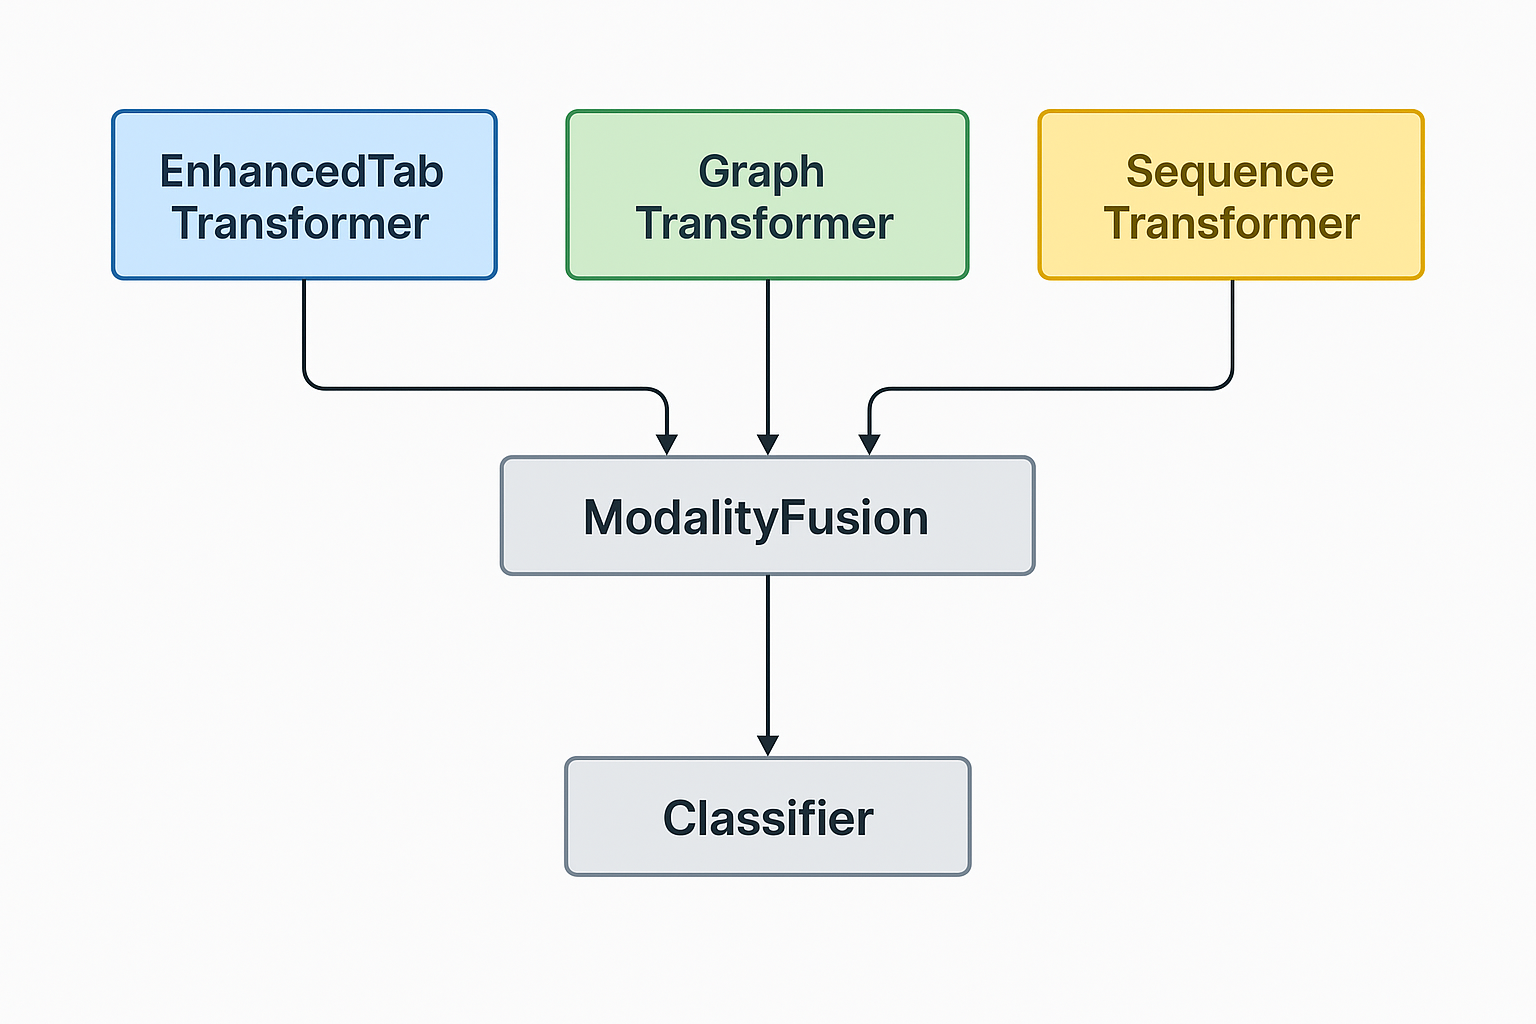
\includegraphics[width=0.9\textwidth]{../images/magnet_architecture.png}
  \caption{Overall Architecture of MAGNET Model}
  \label{fig:architecture}
\end{figure*}

\textbf{EnhancedTabTransformer:} Processes static application characteristics including permissions, components, and manifest metadata. The feature space is reduced to 430 dimensions after preprocessing.

\textbf{GraphTransformer:} Analyzes function call relationships using graph neural networks to capture control flow patterns.

\textbf{SequenceTransformer:} Captures temporal API invocation patterns through sequential analysis.

\subsection{Dynamic Fusion Mechanism}
The final classification leverages a learnable fusion strategy:
\begin{align}
\alpha_i &= \text{softmax}(\mathbf{w}_i^T \tanh(\mathbf{W}_i h_i + \mathbf{b}_i)) \\
\text{Output} &= \sum_{i=1}^{3} \alpha_i \cdot h_i^{\text{fused}}
\end{align}

\section{Experimental Setup}
\subsection{Dataset}
We utilize the DREBIN dataset~\cite{Drebin} comprising 6,092 applications:
\begin{itemize}
  \item \textbf{Training:} 4,641 applications
  \item \textbf{Testing:} 1,451 applications (327 benign, 1,124 malicious)
  \item \textbf{Features:} 430 dimensions after preprocessing
\end{itemize}

\subsection{Hyperparameter Optimization}
We employed dual optimization strategies:
\begin{itemize}
  \item \textbf{PIRATES:} 476 trials → embedding\_dim=32, num\_heads=4, dropout=0.2029
  \item \textbf{Optuna:} 13 trials → embedding\_dim=64, num\_heads=4, dropout=0.2
\end{itemize}

\section{Results}
\subsection{Overall Performance}
MAGNET achieves exceptional performance:
\begin{itemize}
    \item \textbf{Accuracy:} 97.24\%
    \item \textbf{F1-Score:} 0.9823
    \item \textbf{Precision:} 0.9796
    \item \textbf{Recall:} 0.9849
    \item \textbf{AUC:} 0.9932
\end{itemize}

\subsection{Cross-Validation Results}
5-fold cross-validation demonstrates consistent performance:
\begin{table}[!htb]
  \centering
  \caption{5-fold Cross-Validation Results}
  \label{tab:cv_results}
  \begin{tabular}{@{}lccc@{}}
    \toprule
    \textbf{Metric} & \textbf{Mean} & \textbf{Std} & \textbf{Range} \\
    \midrule
    Accuracy & 0.9722 & ±0.0065 & 0.9601-0.9785 \\
    F1-Score & 0.9818 & ±0.0042 & 0.9742-0.9858 \\
    AUC & 0.9932 & ±0.0035 & 0.9861-0.9955 \\
    \bottomrule
  \end{tabular}
\end{table}

\begin{figure}[!htb]
  \centering
  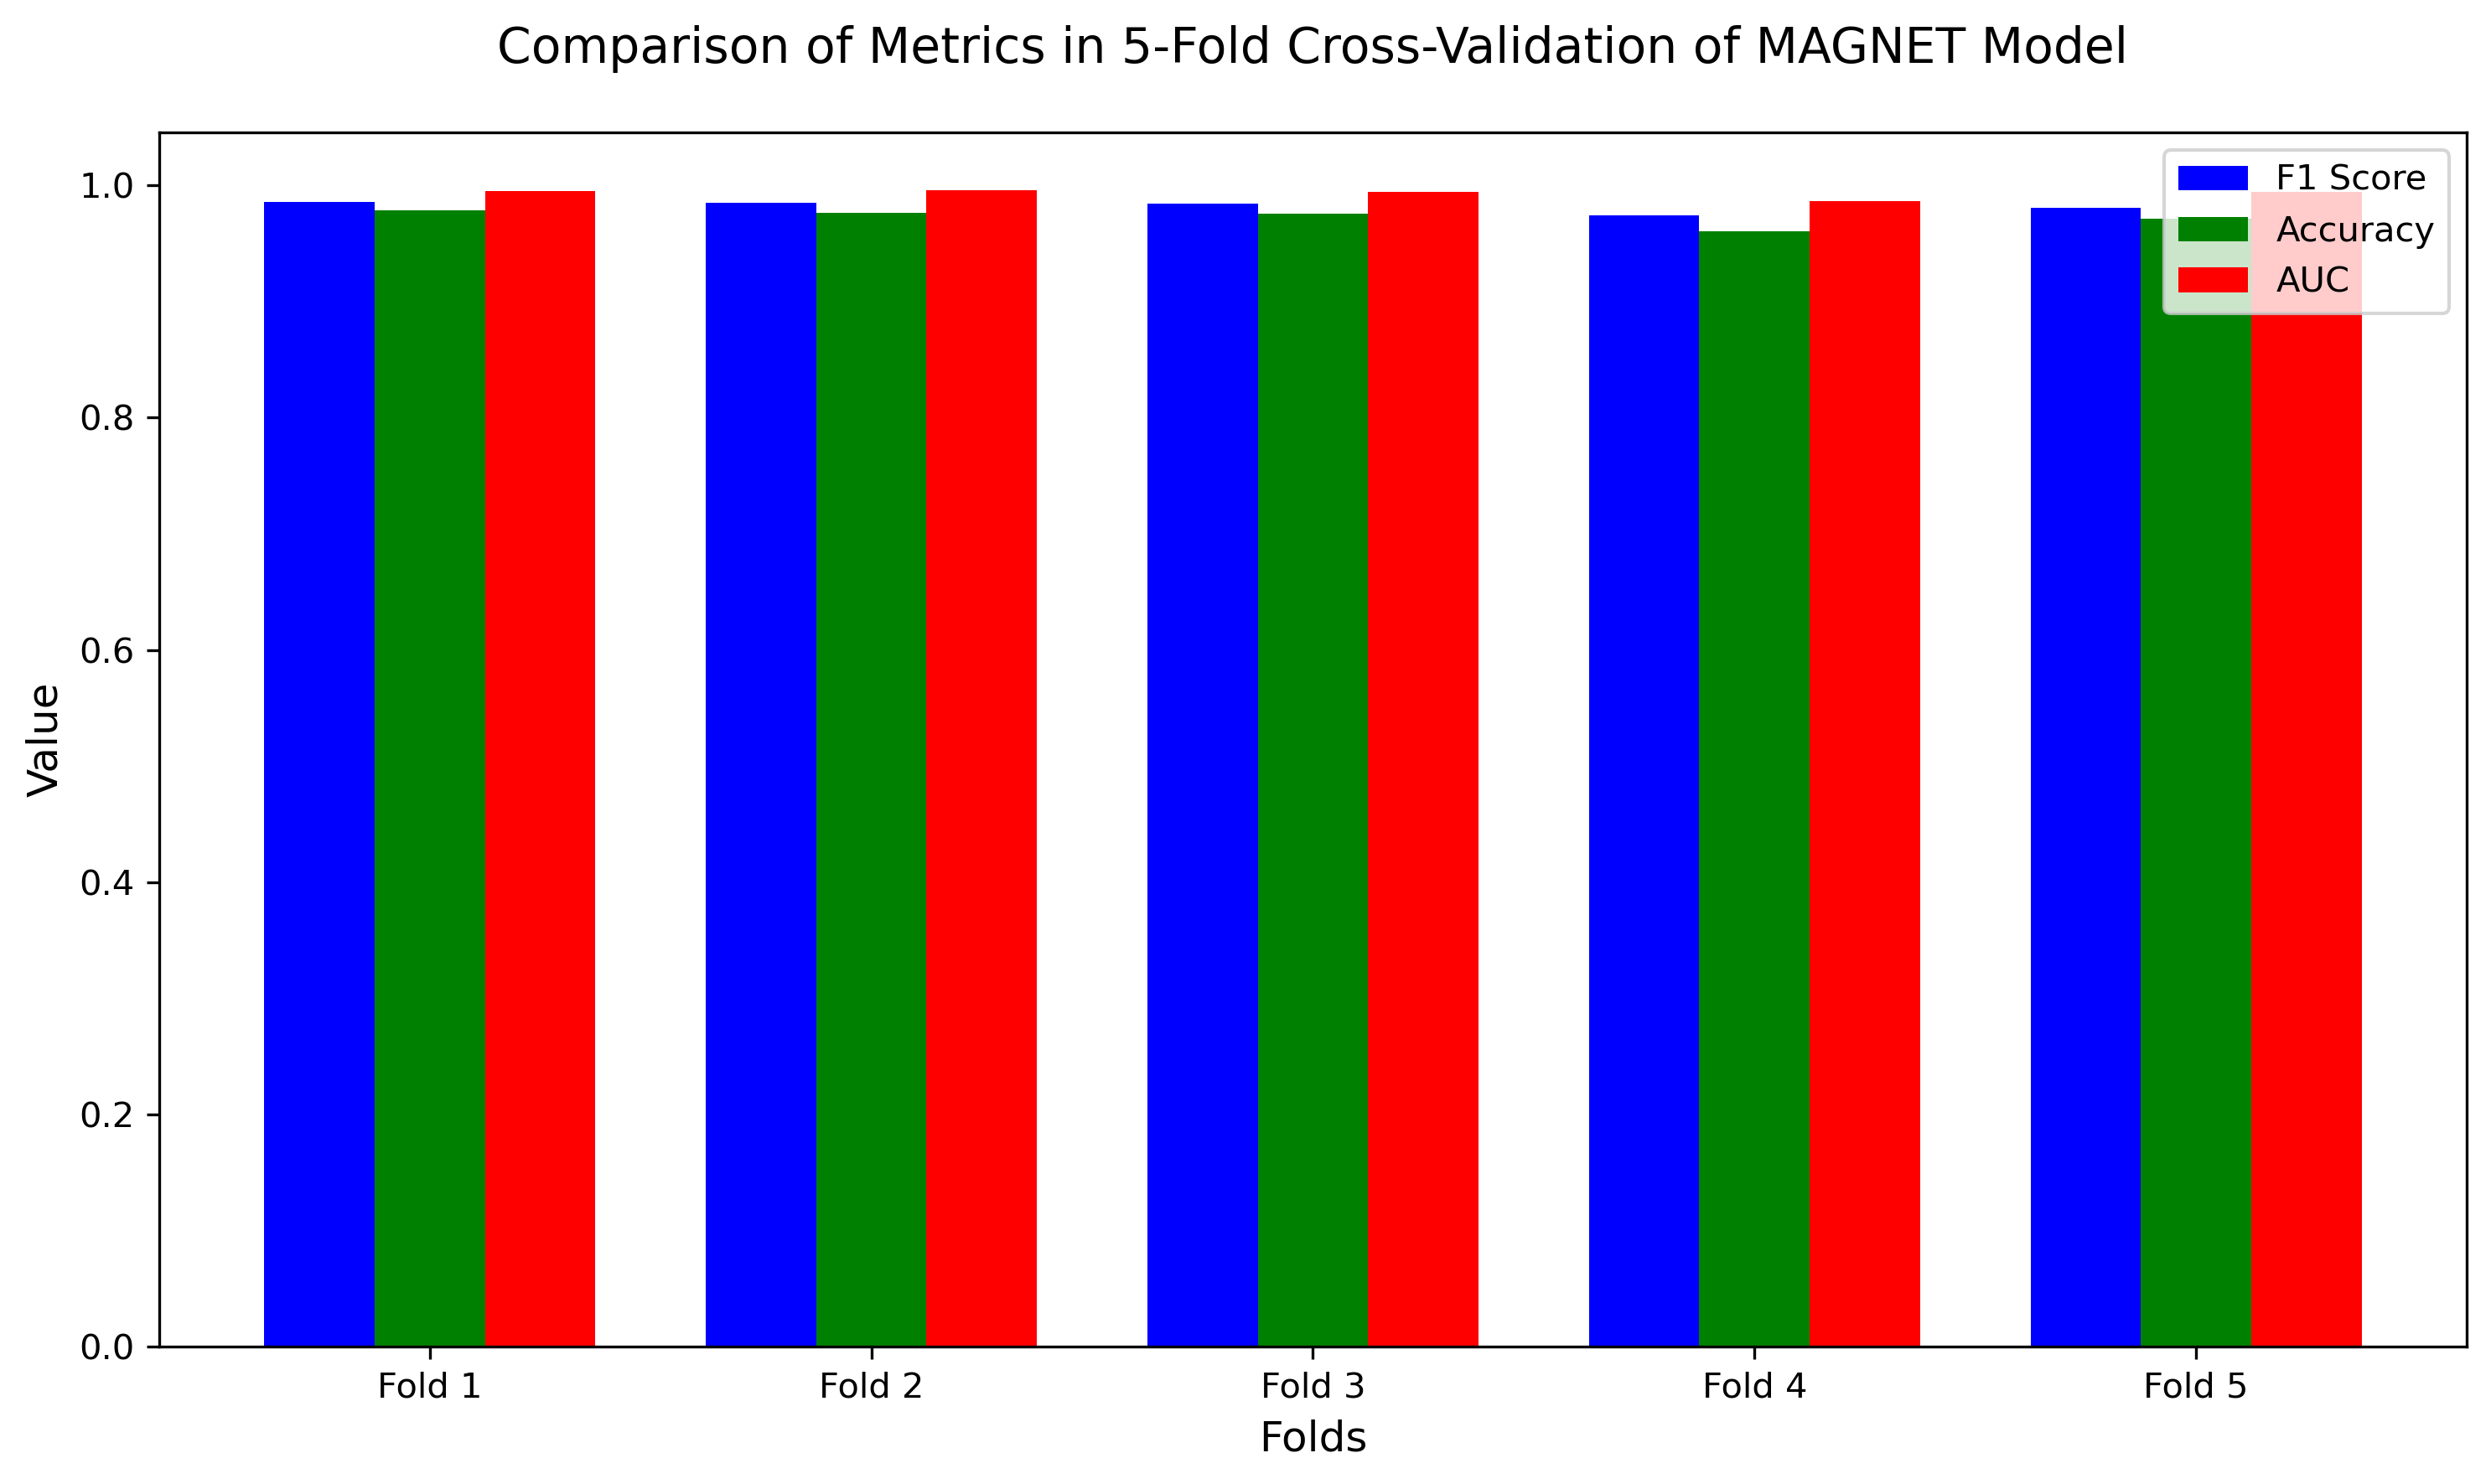
\includegraphics[width=0.9\linewidth]{../fig_cv_metrics.png}
  \caption{Cross-Validation Performance Metrics}
  \label{fig:cv_metrics}
\end{figure}

\subsection{Baseline Comparison}
Table~\ref{tab:baseline_comparison} shows significant improvements over traditional methods:

\begin{table}[!htb]
  \centering
  \caption{Baseline Method Comparison}
  \label{tab:baseline_comparison}
  \begin{tabular}{@{}lccc@{}}
    \toprule
    \textbf{Method} & \textbf{Accuracy} & \textbf{F1-Score} & \textbf{AUC} \\
    \midrule
    SVM & 0.906 & 0.903 & 0.945 \\
    Random Forest & 0.935 & 0.935 & 0.967 \\
    XGBoost & 0.948 & 0.948 & 0.978 \\
    ANN & 0.962 & 0.962 & 0.985 \\
    \midrule
    \textbf{MAGNET} & \textbf{0.972} & \textbf{0.982} & \textbf{0.993} \\
    \bottomrule
  \end{tabular}
\end{table}

\begin{figure}[!htb]
  \centering
  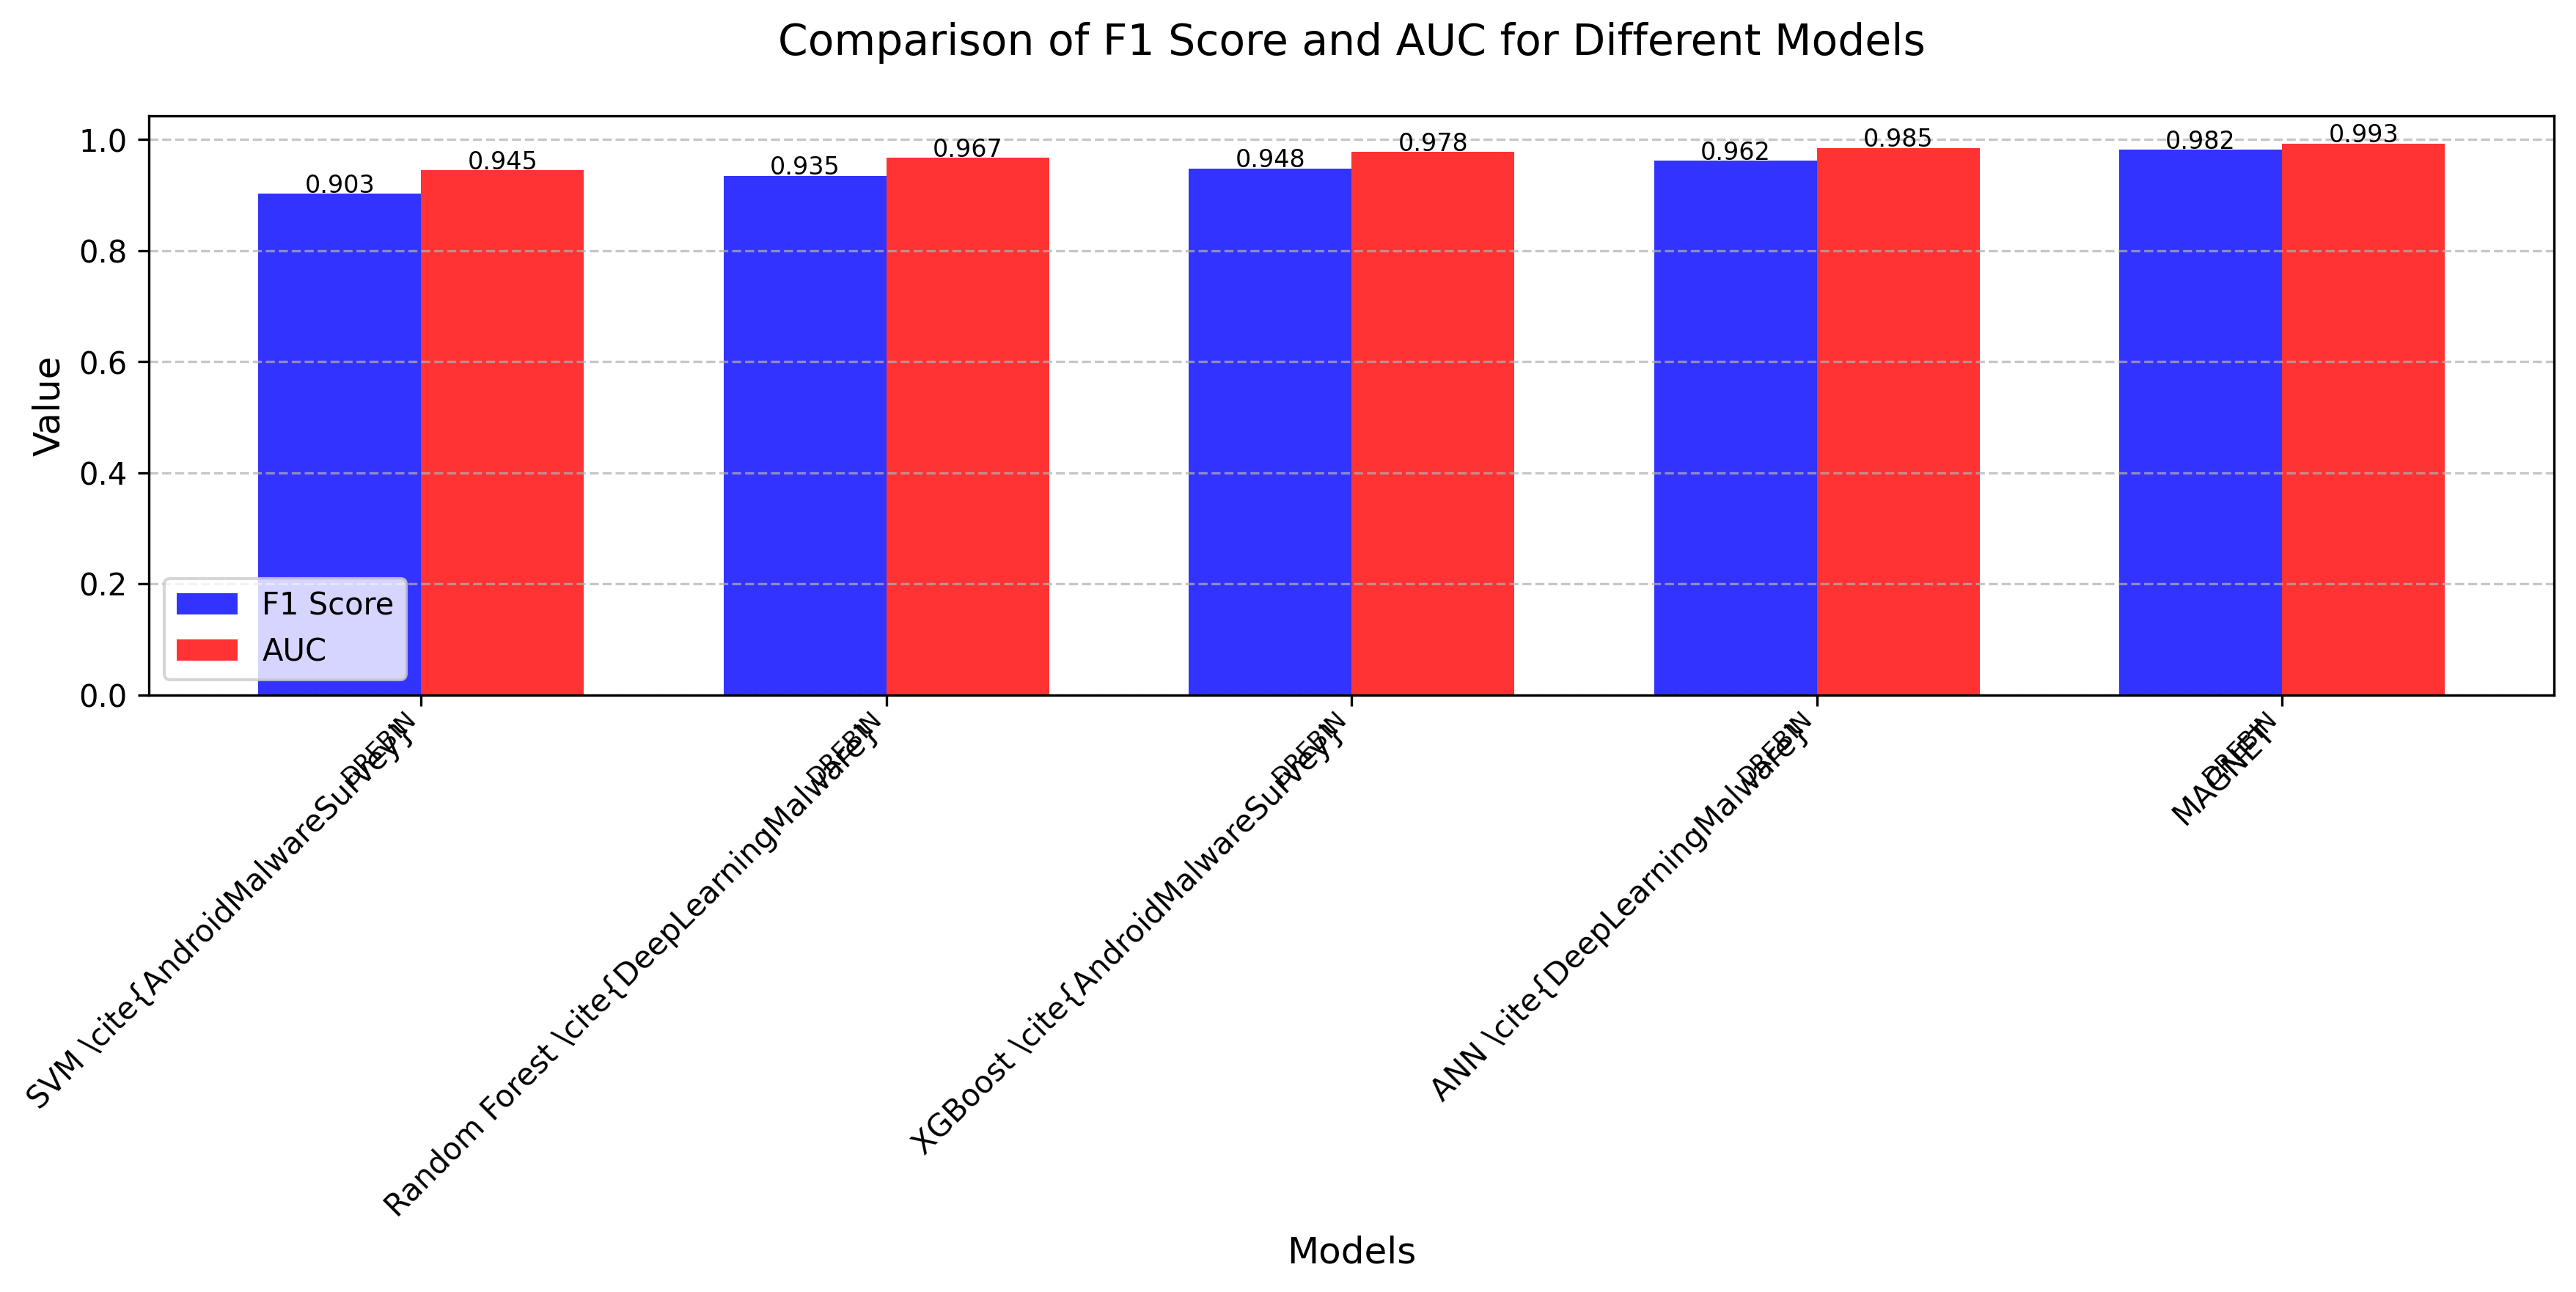
\includegraphics[width=0.9\linewidth]{../fig_baseline_comparison.png}
  \caption{Baseline Method Performance Comparison}
  \label{fig:baseline_comparison}
\end{figure}

\subsection{Component Analysis}
Individual component performance demonstrates complementary contributions:

\begin{table}[!htb]
  \centering
  \caption{Component Performance Analysis}
  \label{tab:component_analysis}
  \begin{tabular}{@{}lc@{}}
    \toprule
    \textbf{Component} & \textbf{F1-Score} \\
    \midrule
    EnhancedTabTransformer & 0.945 \\
    GraphTransformer & 0.894 \\
    SequenceTransformer & 0.907 \\
    \midrule
    Combined (no attention) & 0.954 \\
    Combined (no fusion) & 0.967 \\
    \textbf{MAGNET (Complete)} & \textbf{0.982} \\
    \bottomrule
  \end{tabular}
\end{table}

\begin{figure}[!htb]
  \centering
  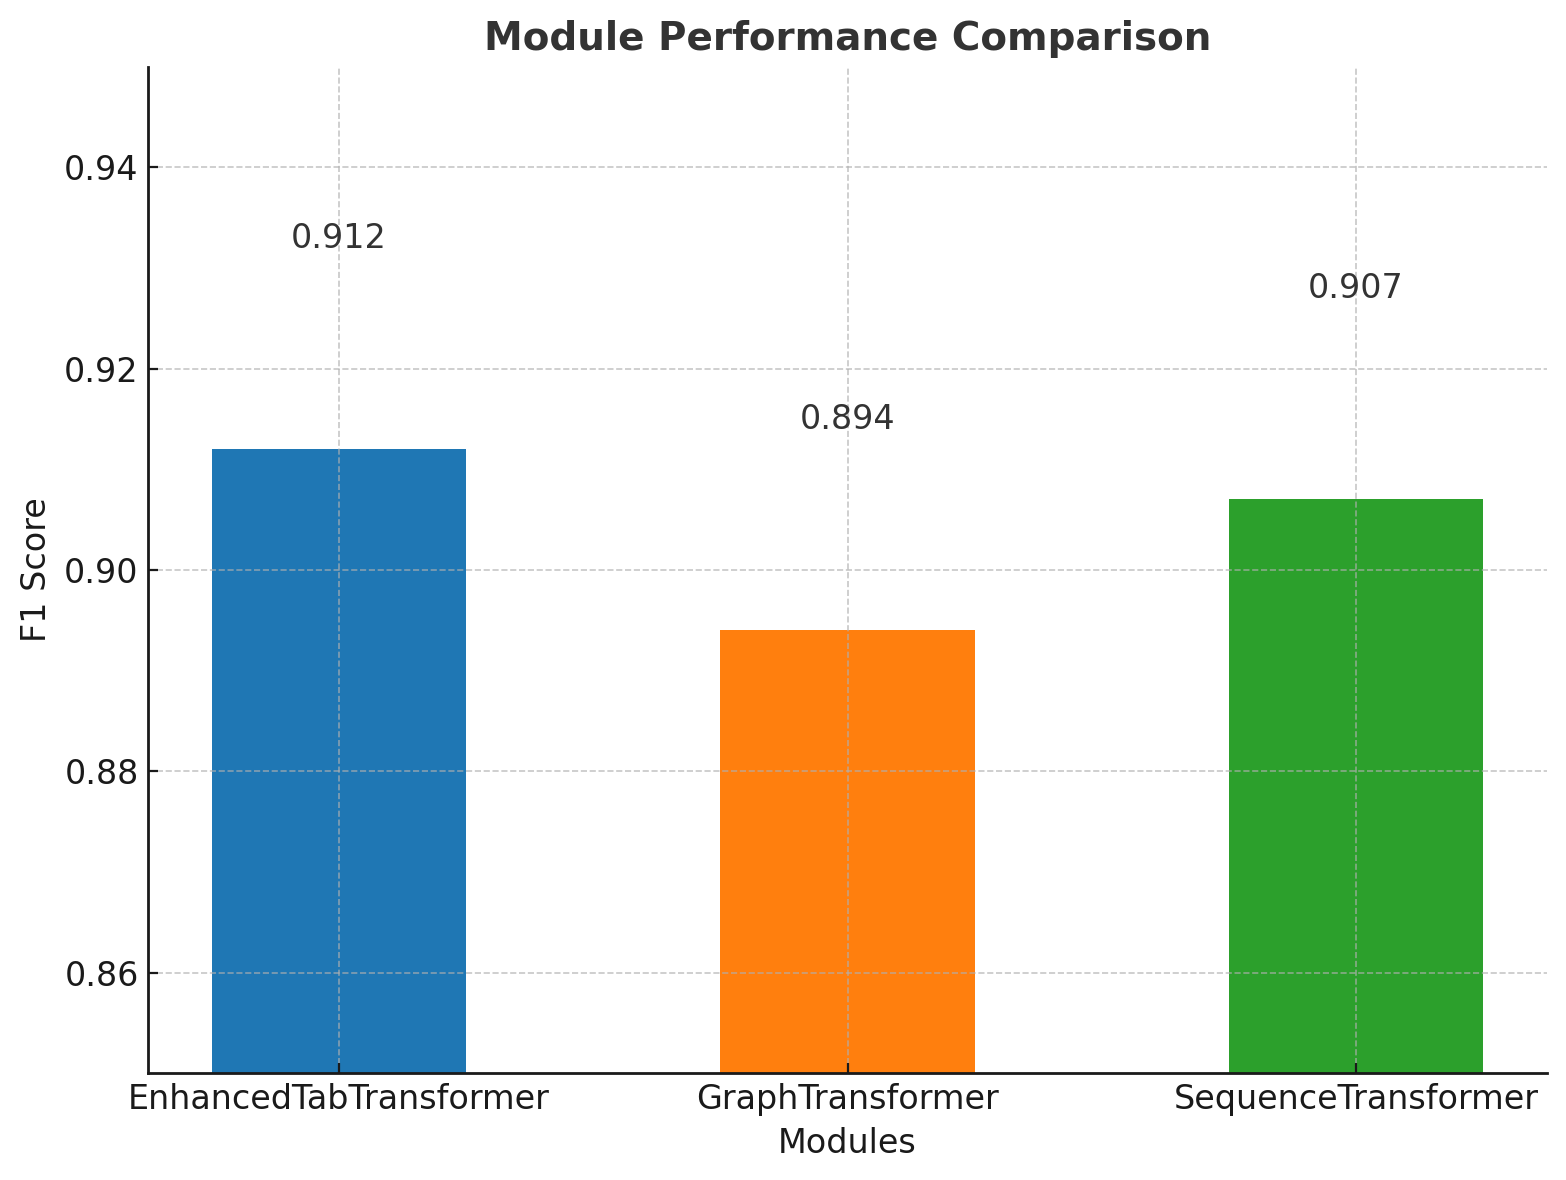
\includegraphics[width=0.9\linewidth]{../images/fig_module_comparison_en.png}
  \caption{Individual Component Performance}
  \label{fig:module_comparison}
\end{figure}

\subsection{State-of-the-Art Comparison}
Table~\ref{tab:literature_comparison} compares MAGNET with recent methods:

\begin{table}[!htb]
  \centering
  \caption{State-of-the-Art Method Comparison}
  \label{tab:literature_comparison}
  \begin{tabular}{@{}lcc@{}}
    \toprule
    \textbf{Method} & \textbf{Accuracy (\%)} & \textbf{F1-Score} \\
    \midrule
    \textbf{MAGNET} & \textbf{97.24} & \textbf{0.9823} \\
    DREBIN (SVM) & 92.3 & 0.933 \\
    PIKADROID & 96.8 & 0.974 \\
    DeepImageDroid & 96.0 & 0.960 \\
    BERT-Graph & 95.5 & 0.950 \\
    Multi-modal & 89.2 & -- \\
    Transformer & 95.8 & -- \\
    \bottomrule
  \end{tabular}
\end{table}

\section{Discussion}
\subsection{Performance Analysis}
MAGNET achieves state-of-the-art performance through several key innovations:

\textbf{Multi-modal Integration:} The synergistic combination of tabular, graph, and sequential modalities creates comprehensive representation spaces. Component analysis shows that tabular features provide the strongest foundation (F1=0.945), while graph and sequential patterns offer complementary information.

\textbf{Dynamic Attention:} The cross-modal attention mechanism contributes significantly by adaptively weighting modality contributions based on input characteristics.

\textbf{Architectural Design:} Single-layer transformers with optimized hyperparameters achieve optimal performance while maintaining computational efficiency.

\subsection{Comparative Analysis}
MAGNET demonstrates significant improvements:
- +6.64\% over SVM
- +3.74\% over Random Forest
- +2.44\% over XGBoost
- +1.04\% over ANN

Compared to recent methods, MAGNET outperforms PIKADROID (+0.44\%), DeepImageDroid (+1.24\%), and BERT-Graph (+1.74\%).

\subsection{Limitations}
Several limitations warrant consideration:
\begin{itemize}
    \item Computational requirements may limit real-time deployment
    \item Dataset temporal scope (2010-2014) may affect generalization
    \item Need for sophisticated preprocessing across modalities
\end{itemize}

\section{Conclusion}
We present MAGNET, a novel multi-modal framework for Android malware detection achieving state-of-the-art performance with 97.24\% accuracy and F1-score of 0.9823. The key contributions include:

\begin{itemize}
    \item Unified multi-modal architecture with three specialized processing modules
    \item Dynamic attention mechanism for optimal information fusion
    \item Comprehensive evaluation demonstrating superior performance
    \item Practical applicability for operational security systems
\end{itemize}

Our ablation studies confirm that each component contributes meaningfully to overall performance. The model's superior results and robust evaluation make it suitable for production deployment.

Future work should focus on:
\begin{itemize}
    \item Evaluation on contemporary datasets
    \item Model compression for resource-constrained environments
    \item Investigation of adversarial robustness
    \item Extension to other platforms and malware types
\end{itemize}

\onecolumn
\newpage
\printbibliography[heading=bibintoc,title={References}]

\end{document}
